\documentclass[shownotes,11pt, aspectratio=169]{beamer}

\usepackage{pgfpages}
\setbeameroption{hide notes} % Only slide
%\setbeameroption{show only notes} % Only notes
%\setbeameroption{show notes on second screen=right} % Both

\usepackage{helvet}
\usepackage[default]{Fira Sans}
\usepackage{array}
\usepackage{caption}
%\usepackage[clean]{svg}
\usepackage{tikz}
\usepackage{verbatim}
\setbeamertemplate{note page}{\pagecolor{yellow!5}\insertnote}
\usetikzlibrary{positioning}
\usetikzlibrary{snakes}
\usetikzlibrary{calc}
\usetikzlibrary{arrows}
\usetikzlibrary{decorations.markings}
\usetikzlibrary{shapes.misc}
\usetikzlibrary{matrix,shapes,arrows,fit,tikzmark}
\usepackage{amsmath}
\usepackage{mathpazo}
\usepackage{hyperref}
\usepackage{lipsum}
\usepackage{multimedia}
\usepackage{graphicx}
\usepackage{multirow}
\usepackage{graphicx}
\usepackage{dcolumn}
\usepackage{bbm}
\newcolumntype{d}[0]{D{.}{.}{5}}

\usepackage{changepage}
\usepackage{appendixnumberbeamer}
\newcommand{\beginbackup}{
   \newcounter{framenumbervorappendix}
   \setcounter{framenumbervorappendix}{\value{framenumber}}
   \setbeamertemplate{footline}
   {
     \leavevmode%
     \hline
     box{%
       \begin{beamercolorbox}[wd=\paperwidth,ht=2.25ex,dp=1ex,right]{footlinecolor}%
%         \insertframenumber  \hspace*{2ex} 
       \end{beamercolorbox}}%
     \vskip0pt%
   }
 }
\newcommand{\backupend}{
   \addtocounter{framenumbervorappendix}{-\value{framenumber}}
   \addtocounter{framenumber}{\value{framenumbervorappendix}} 
}


\usepackage{graphicx}
\usepackage[space]{grffile}
\usepackage{booktabs}

\definecolor{blue}{RGB}{0,114,178}
\definecolor{red}{RGB}{213,94,0}
\definecolor{yellow}{RGB}{240,228,66}
\definecolor{green}{RGB}{0,158,115}

\hypersetup{
  bookmarks=true,
  colorlinks=false,
  linkbordercolor = {white},
  linkcolor = {blue}
}


%% I use a beige off white for my background
\definecolor{MyBackground}{RGB}{255,253,218}

%% Uncomment this if you want to change the background color to something else
\setbeamercolor{background canvas}{bg=MyBackground}

%% Change the bg color to adjust your transition slide background color!
\newenvironment{transitionframe}{
  \setbeamercolor{background canvas}{bg=yellow}
  \begin{frame}}{
    \end{frame}
}

\setbeamercolor{frametitle}{fg=blue}
\setbeamercolor{title}{fg=black}
\setbeamertemplate{footline}[frame number]
\setbeamertemplate{navigation symbols}{} 
\setbeamertemplate{itemize items}{-}
\setbeamercolor{itemize item}{fg=blue}
\setbeamercolor{itemize subitem}{fg=blue}
\setbeamercolor{enumerate item}{fg=blue}
\setbeamercolor{enumerate subitem}{fg=blue}
\setbeamercolor{button}{bg=MyBackground,fg=blue,}



\setbeamercolor{section in toc}{fg=blue}
\setbeamercolor{subsection in toc}{fg=red}
\setbeamersize{text margin left=1em,text margin right=1em} 

\newenvironment{wideitemize}{\itemize\addtolength{\itemsep}{10pt}}{\enditemize}

\title[]{\textcolor{blue}{Macroeconomics: Lecture 1}}
\author[SM]{Sumit Mishra}
\institute[IFMR]{\small{\begin{tabular}{c}
IFMR, Sri City \\
\end{tabular}}}

\date{23 September, 2019}


\begin{document}

%%% TIKZ STUFF
\tikzset{   
        every picture/.style={remember picture,baseline},
        every node/.style={anchor=base,align=center,outer sep=1.5pt},
        every path/.style={thick},
        }
\newcommand\marktopleft[1]{%
    \tikz[overlay,remember picture] 
        \node (marker-#1-a) at (-.3em,.3em) {};%
}
\newcommand\markbottomright[2]{%
    \tikz[overlay,remember picture] 
        \node (marker-#1-b) at (0em,0em) {};%
}
\tikzstyle{every picture}+=[remember picture] 
\tikzstyle{mybox} =[draw=black, very thick, rectangle, inner sep=10pt, inner ysep=20pt]
\tikzstyle{fancytitle} =[draw=black,fill=red, text=white]
%%%% END TIKZ STUFF

% Title Slide
\begin{frame}
\maketitle
\end{frame}

\section{Getting Started}
%%SLIDE 1
\begin{frame}
\begin{wideitemize}
\item What is macroeconomics
\item An outline of this course
\item The macroeconomics of the short run
\item The macroeconomics of the long run
\item Basic analytical tools. 
\end{wideitemize}
\end{frame}

%%SLIDE 2
\begin{frame}
\frametitle{What is Macroeconomics?}
\begin{wideitemize}
\item Why is an average Indian today more than \textcolor{green}{20 times richer} than the average Indian some 60 years ago?
\item Why is an average American 50 times richer than an average Ethiopian today?
\item Why is the gap between Indian and South Korean GDP in 2016 \textcolor{red}{nearly twice} of what it was in 1960?
\item What is GDP and how is it measured?
\item What determines the inflation rate?
\item How is the level of unemployed determined?
\item What is the role of government in crisis?
\item Is financialization of economy \textcolor{red}{any good}?
\end{wideitemize}
\end{frame}

%%SLIDE 3
\begin{frame}
\frametitle{Course Structure}
\begin{wideitemize}
\item[1] The Short Run
     \begin{wideitemize}
      \item What causes recessions and booms?
      \item Monetary and fiscal policies.
      \item The crises- global financial crisis, Lira crisis.
      \item Exchange rate management and international financial system.
      \end{wideitemize}
\item[2] The Long Run
       \begin{wideitemize}
        \item Why are some countries richer than others?
        \item What are the sources of economic growth?
         \item What does the relationship between inflation and output look like in a longer horizon?
         \item How trade dynamics change over time?
         \end{wideitemize}
\end{wideitemize}
\end{frame}

%%SLIDE 4
\begin{frame}
\frametitle{Course Logistics}
 Course Material, Resources, and Other Pre-requisites:
    \begin{wideitemize}
     \item Primary text: Blanchard, Macroeconomics.
     \item Lecture slides, handouts, readings, and notes.
     \item Database on Indian Economy, RBI \\
           (Link: \url{https://dbie.rbi.org.in/DBIE/dbie.rbi?site=home})
     \item World Bank Database \\
           (Link: \url{https://data.worldbank.org/})
      \pause
     \item Required reading: \textit{The Economist}, \textit{The Financial Times}
      \pause
     \item Announced and unannounced quizzes, assignments.
     \item One presentation on contemporary economic issues.
     \end{wideitemize}
\end{frame}

%%SLIDE 5
\begin{frame}
\frametitle{Course Logistics}
\begin{wideitemize}
       \item Office hours: Tuesday (3pm-4pm) (Office \# 223 )
       \item Phone: +91-750-682-4634
       \pause
      \item TA: \textbf{} (They will announce their office hours later.)
\end{wideitemize}
\end{frame}

%%SLIDE 7
\begin{frame}
\frametitle{Course Logistics}
\begin{wideitemize}
\item Review the syllabus.
\item Four to six assignments (mostly or entirely unannounced and in-class).
\item Dropbox will contain all that you need.
\item No electronic devices while you are in class.
\item Be reasonable and decent w.r.t. attendance policy. 
\end{wideitemize}
\end{frame}

%%SLIDE 8
\begin{frame}
\frametitle{Evaluation and Grading}
\begin{wideitemize}
\item One mid-term examination (30\%)
\item One final exam (30\%)
\item In-class tests, quizzes, assignments (15\%)
\item One project report/presentation (25\%)
\end{wideitemize}
\end{frame}

%%SLIDE 9
\begin{frame}
\frametitle{Jargon Begins}
\begin{figure}[ht]
%\renewcommand{\thefigure}{A2.1} 
%\captionsetup{labelformat=empty} 
  \caption*{GDP Smackdown}
  %\begin{subfigure}[b]{0.5\linewidth}
   % \centering
   % 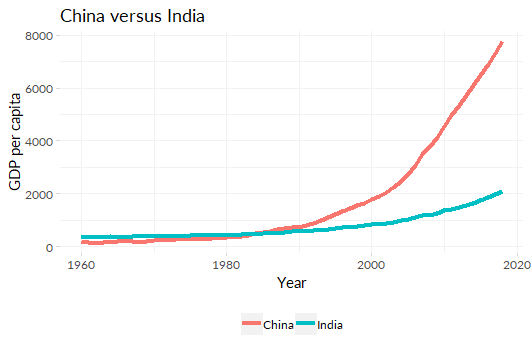
\includegraphics[width=.75\linewidth]{graphs/L012019F02.png} 
     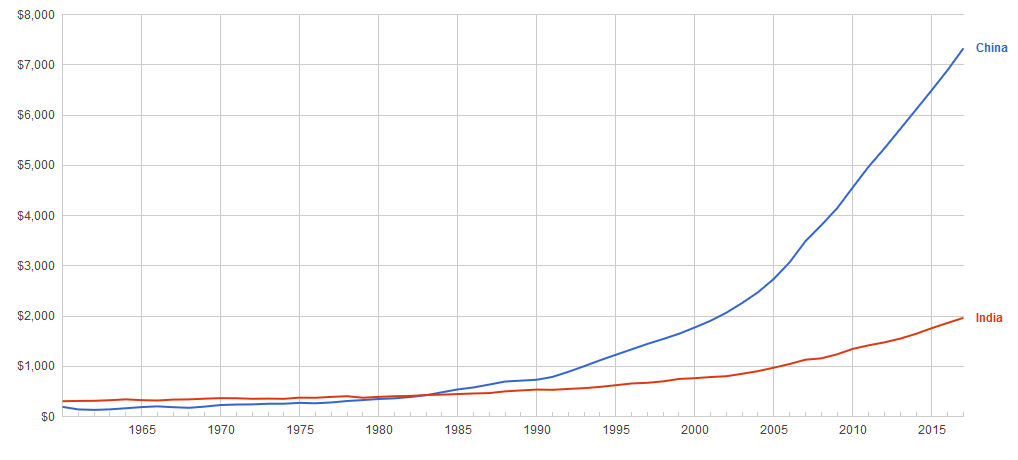
\includegraphics[width=.95\linewidth]{graphs/L1F1.png}    
    \end{figure}\end{frame}

%%SLIDE 10
\begin{frame}
\frametitle{Jargon Continues}
\begin{figure}[ht]
%\renewcommand{\thefigure}{A2.1} 
%\captionsetup{labelformat=empty} 
  \caption*{GDP Growth Rate: India}
  %\begin{subfigure}[b]{0.5\linewidth}
   % \centering
    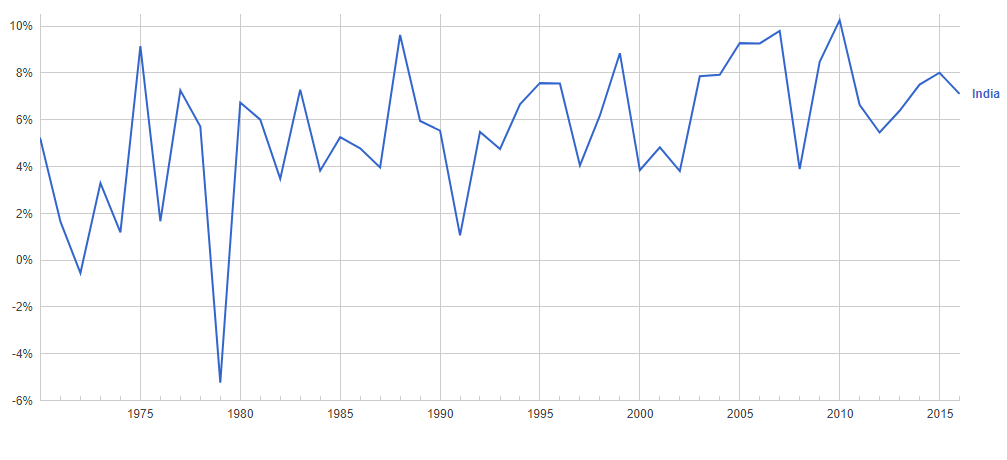
\includegraphics[width=.95\linewidth]{graphs/Growth_Rate_India.png} 
    \end{figure}
\end{frame}

%%SLIDE 11
\begin{frame}
\frametitle{Jargon Continues}
\begin{figure}[ht]
%\renewcommand{\thefigure}{A2.1} 
%\captionsetup{labelformat=empty} 
  \caption*{Inflation: India \\
           1990-2016}
\resizebox{0.5\linewidth}{!}{
    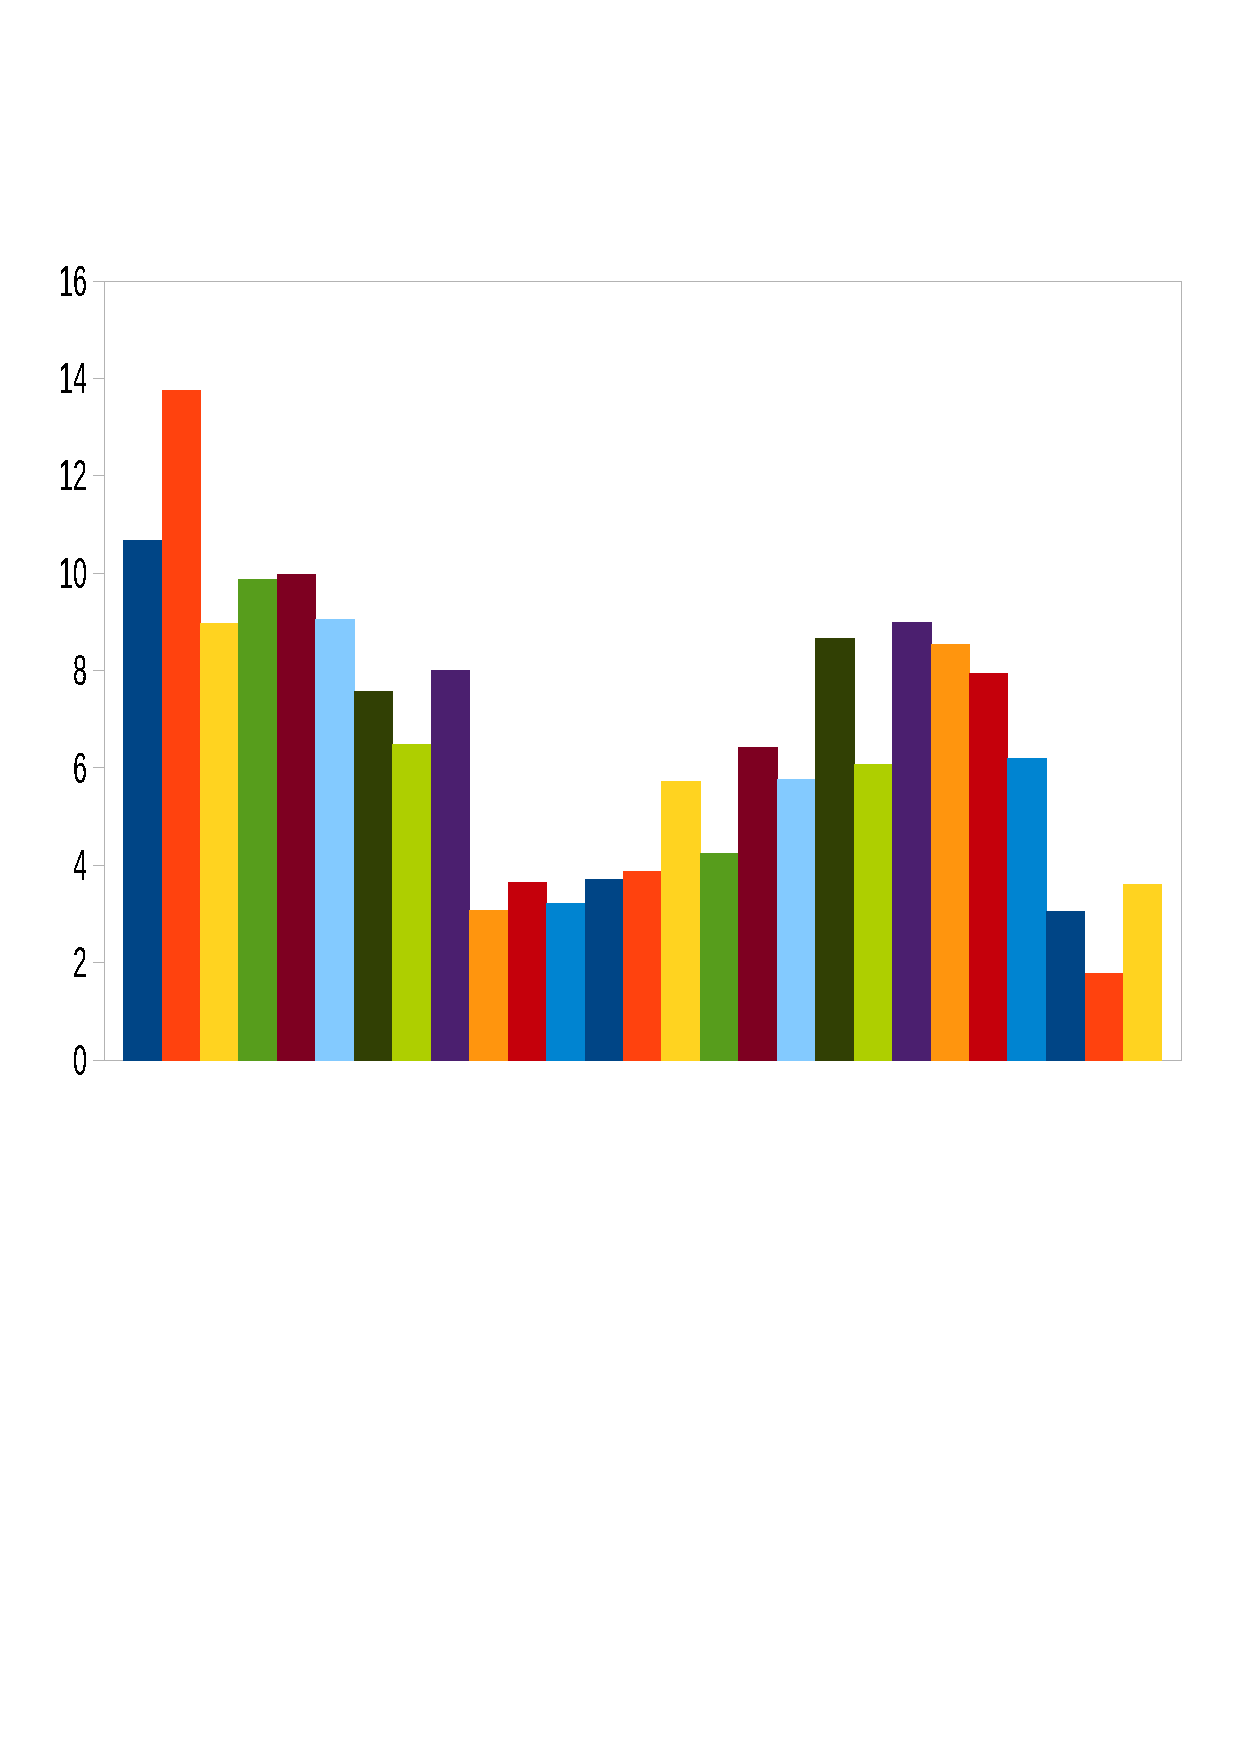
\includegraphics[width=.65\linewidth]{graphs/Inflation_India.pdf}}
    \end{figure}
\end{frame}

%%SLIDE 12

\begin{frame}
%\frametitle{Jargon Continues}
\begin{figure}[ht]
%\renewcommand{\thefigure}{A2.1} 
%\captionsetup{labelformat=empty} 
  \caption*{Per-capita GDP Across the Universe}
    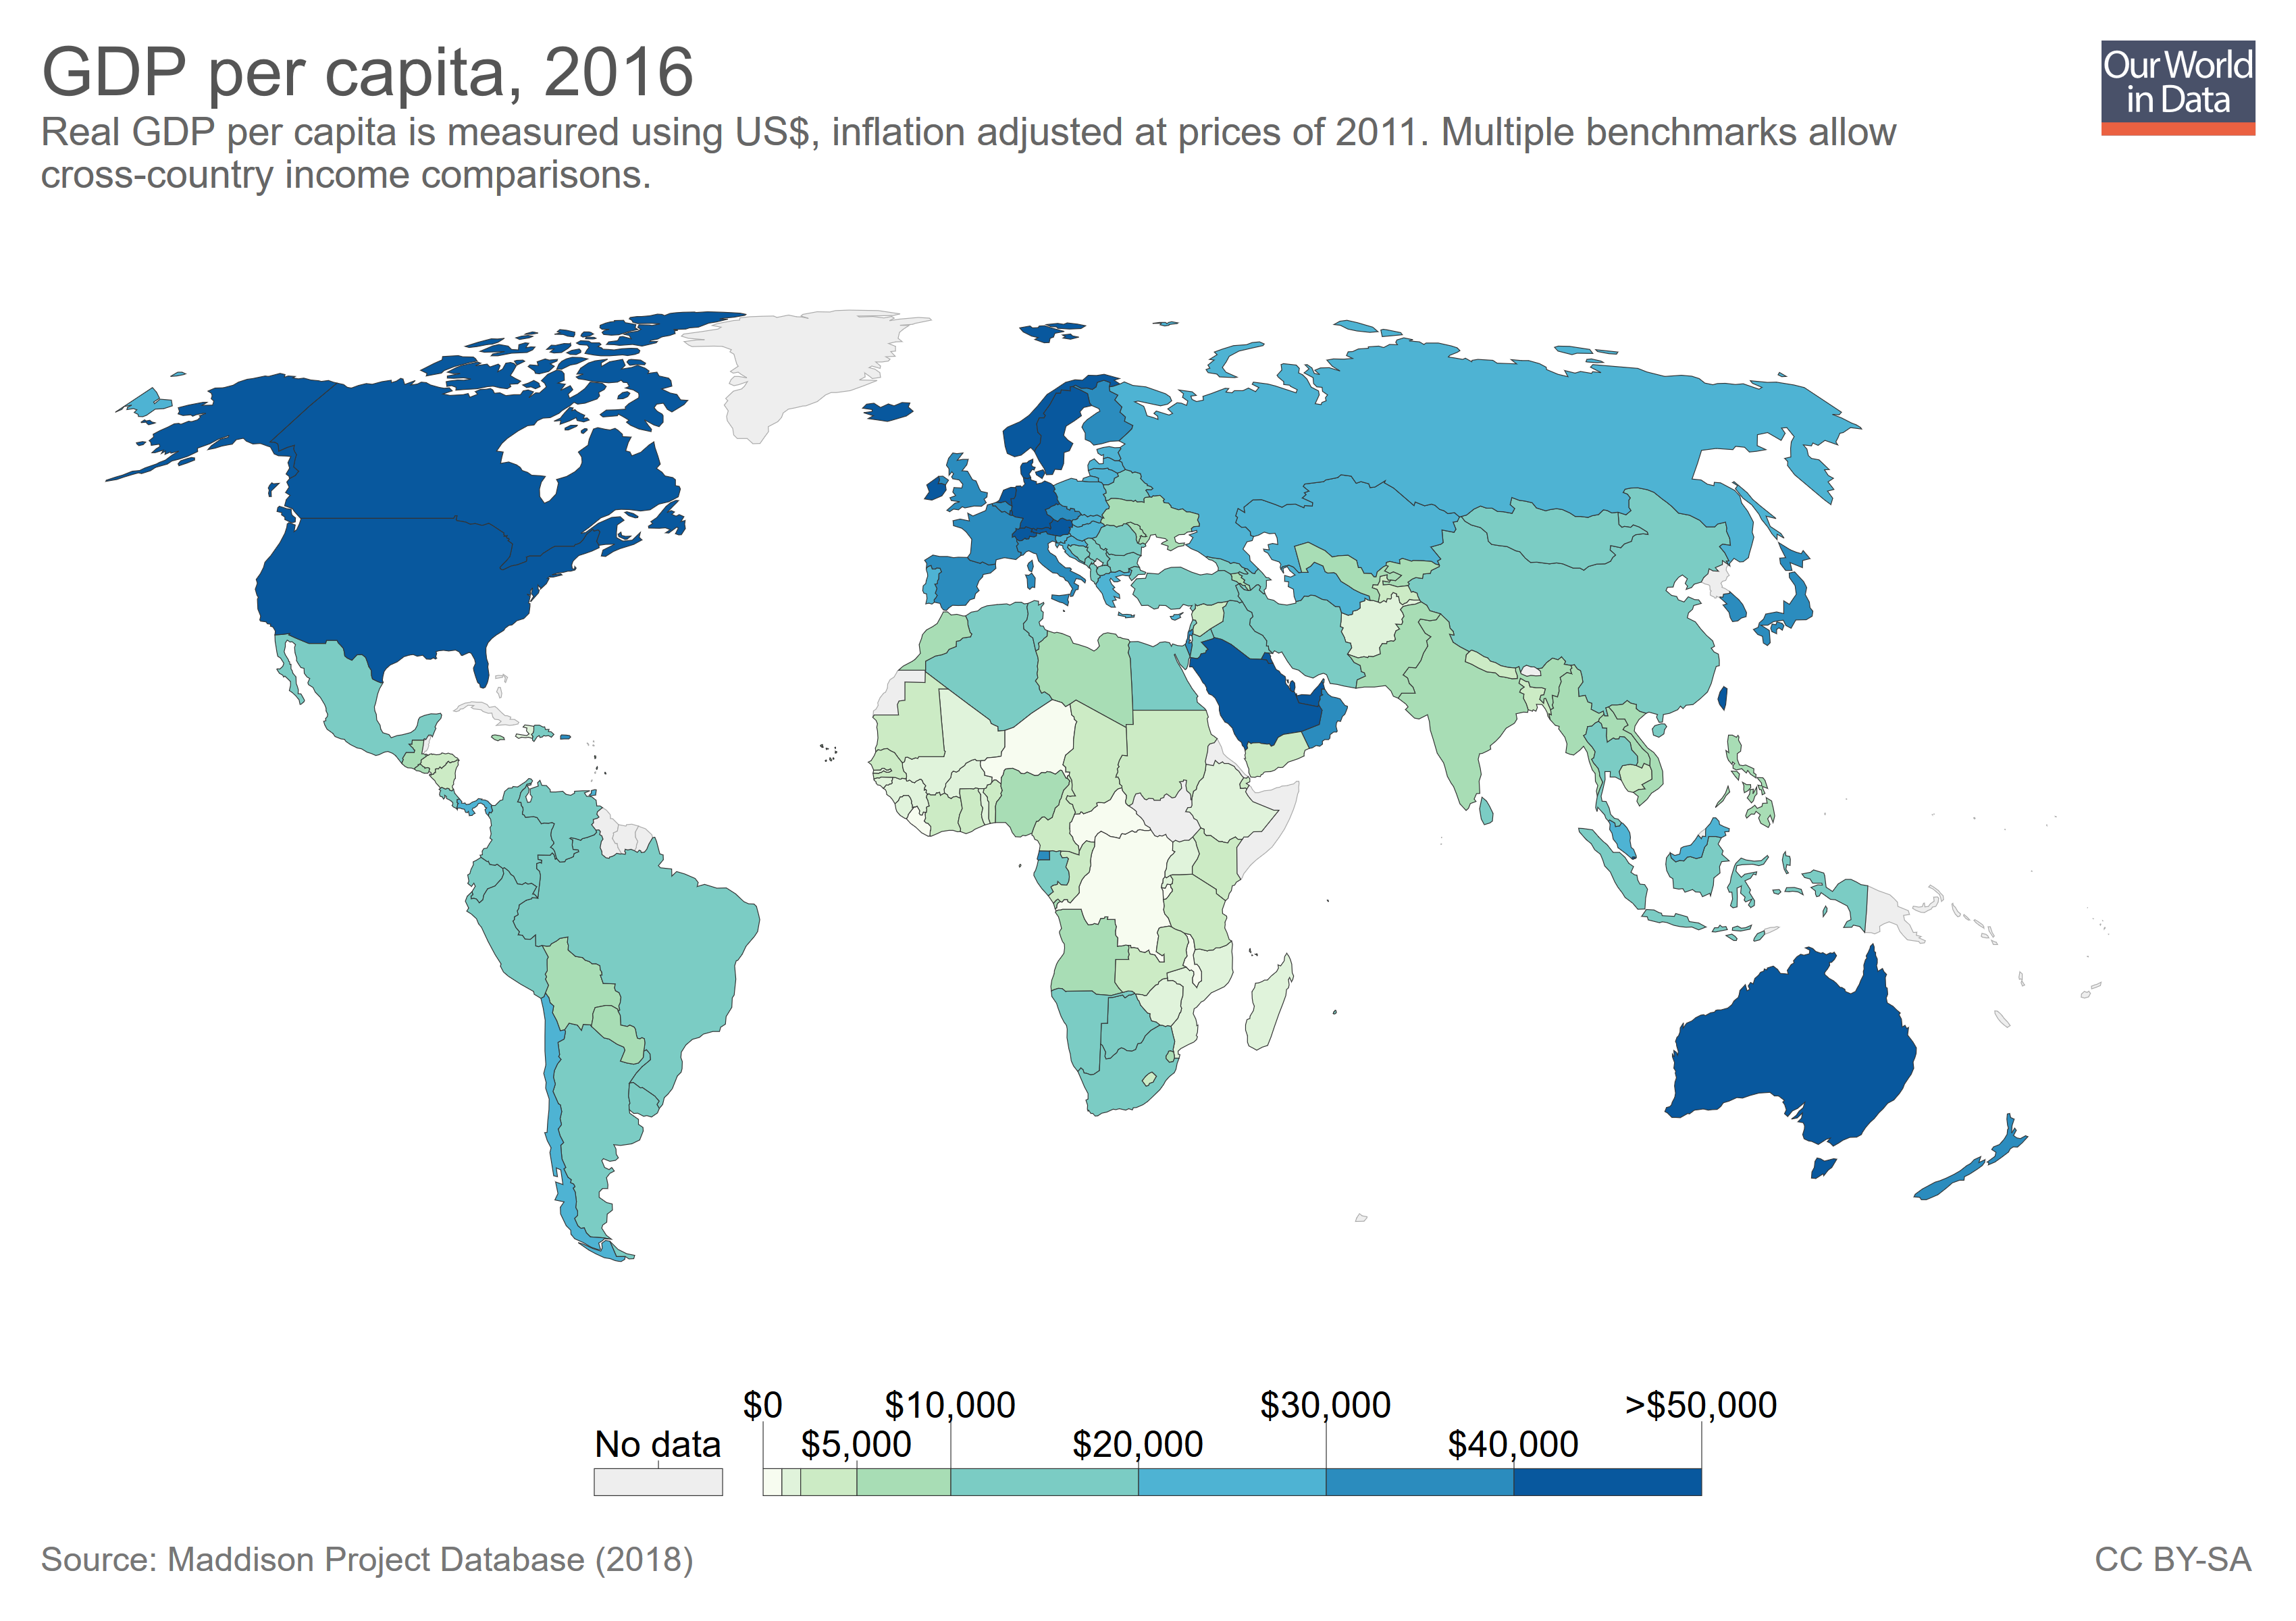
\includegraphics[width=.95\linewidth]{graphs/L1F8.png}
    \end{figure}
\end{frame}



%%SLIDE 13
\begin{frame}
\frametitle{Cookbook: Models, Data, and Discussions}
\begin{wideitemize}
\item \textcolor{red}{Document facts}
\item \textcolor{green}{Think through a model (a fable)}
\item Does the model explain the world?
\end{wideitemize}
\end{frame}

%%
\begin{frame}{The Indian Story}
\begin{figure}
\resizebox{0.55\linewidth}{!}{
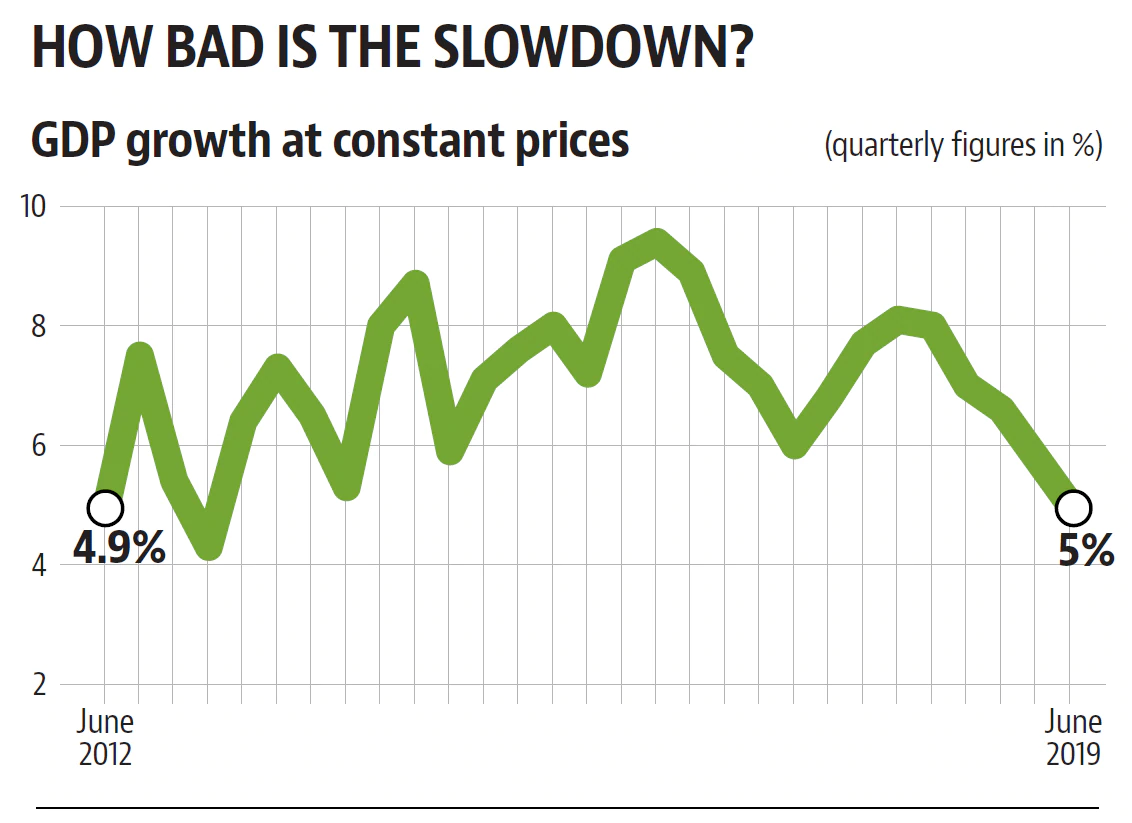
\includegraphics{graphs/L012019F01.png}}
\end{figure}
\textbf{Source:} \url{https://www.hindustantimes.com/editorials/state-of-economy-in-10-charts/story-825WukaxZqGI09QM0z2NlJ.html}
\end{frame}

\section{Going Back to the Start (Microeconomics)}
\begin{frame}{Side Effects of Market Concentration}
\begin{wideitemize}
\item Low productivity, slow wage growth are somehow linked to rising market concentration.
\item Alan Krueger of Princeton blames: employers' clout (no-poaching agreements), lack of unions, and falling value of minimum wages.
\pause
\item  Platforms such as Google, Uber and Airbnb match buyers and sellers, and thus make outsize gains as they grow. 
\item In such winner-takes-most competition, a slight advantage can tip the entire market in a company's favour.
\end{wideitemize}
\textbf{Source:} \url{https://www.economist.com/finance-and-economics/2018/08/30/central-bankers-grapple-with-the-changing-nature-of-competition}
\end{frame}

\begin{frame}{Side Effects of Market Concentration}
\begin{wideitemize}
\item Concentration means high consumer prices and lower wages.
\item Firms squeeze greater profits.
\item Some studies show that high markups can be extremely detrimental to consumers.
\item Economists are sounding alarm on the threat posed by corporate power.
\end{wideitemize}
\textbf{Source:} \url{https://www.bloomberg.com/view/articles/2018-09-04/economists-gear-up-to-challenge-the-monopolies}
\end{frame}

%%%
\begin{frame}{Market Concentration and Macroeconomics}
\begin{wideitemize}
\item Financial wealth has increased rapidly despite no real increase in the amount of investment in the economy.
\item This rise in wealth hasn't translated into greater investments.
\item Interest rates have fallen, but average rate of return on capital has remained steady.
\item The share of labour income has declined. 
\item An increase in monopoly rent has driven up the returns on capital.
\end{wideitemize}
\textbf{Source:} \url{https://equitablegrowth.org/how-the-rise-of-market-power-in-the-united-states-may-explain-some-macroeconomic-puzzles/}
\end{frame}



%%SLIDE 1
\begin{frame}
\frametitle{Agenda}
\begin{itemize}
\item Measuring National Income
\item Measuring Cost of Living
%\item Measuring Unemployment
%\item Goods Market
%\item Material: Blanchard, Chapters 2, 3.
\end{itemize}
\end{frame}

\section{GDP: Primer}
\begin{frame}
\textbf{Gross Domestic Product (GDP)} \\

\vspace{3mm}

\textit{The market value of all final goods and services produced \textcolor{red}{within a country} in a \textcolor{red}{given period of time}.}

\end{frame}

\begin{frame}
\textbf{Market Value} \\

\vspace{3mm}

\textit{GDP adds together many different kinds of products into a single measure of the value of economic activity. To do this, it uses market prices. Because market prices measure the amount people are willing to pay for
different goods, they reflect the value of those goods. If the price of an apple is twice the price of an orange, then an apple contributes twice as much to GDP as does an orange.}

\end{frame}

\begin{frame}
\textbf{Of All?} \\
\vspace{2mm}

GDP measures the market value of not just apples and oranges but also mangoes and jackfruits, books and movies, haircuts and healthcare, and on and on. \\
\vspace{2mm}

\pause

GDP also includes the market value of the housing services provided by the economy's stock of housing. For rental housing, this value is easy to calculate- the rent equals both the tenant's expenditure and the landlord's income. Yet many people own the place where they live and, therefore, do not pay rent.\\
How would you then measure GDP?

\end{frame}

\begin{frame}
\textbf{Of All?} \\
Not really. There are goods and services that can't be included in GDP. \\
Examples? \\
\vspace{2mm}
\pause

Household chores are not included in GDP.
\end{frame}

\begin{frame}
\textbf{Final Goods} \\
\vspace{2mm}

The coffee procured by Blue Tokai from a coffee plantation in Karnataka is an \textit{intermediate good}.
The cappuccino or macchiato you get in the end is the \textit{final good}. \\
The GDP only accounts for the value of final good. Why? 
\\
\vspace{3mm}

This is done because the value of intermediate goods is already included in the prices of the final goods.
\end{frame}

\begin{frame}
\textbf{Goods and Services}
\\
\vspace{3mm}

\textit{GDP includes both tangible goods (food, clothing, cars) and intangible services
(haircuts, housecleaning, doctor visits). When you buy a CD by your favourite
band, you are buying a good, and the purchase price is part of GDP. When you
pay to hear a concert by the same band, you are buying a service, and the ticket
price is also part of GDP.}

\end{frame}


\begin{frame}
\textbf{Produced}
\\
\vspace{3mm}

GDP includes goods and services currently produced. It does not include transactions
involving items produced in the past. When Motorola produces and
sells a new phone, the value of the phone is included in GDP. When you decide to sell it on OLX, the value of the used Motorola phone is not included in GDP.
\end{frame}


\begin{frame}
\textbf{Within the country}
\\

\vspace{3mm}

GDP measures the value of production within the geographic confines of a country.
\begin{itemize}
\item When an Indian citizen works temporarily in the United States, her income is part of U.S. GDP. 
\item When an American citizen owns a factory in India, the production at his factory is not part of U.S. GDP. 
\item Thus, items are included in a nation's GDP if they are produced domestically, regardless
of the nationality of the producer.
\end{itemize}
\end{frame}

\begin{frame}
\textbf{In a given time period}\\
\vspace{3mm}

GDP measures the value of production that takes place within a specific interval
of time. 
\begin{itemize}
\item Usually, that interval is a year or a quarter (three months). GDP measures
the economy's flow of income and expenditure during that interval.
\item When the government reports the GDP for a quarter, it usually presents GDP
``at an annual rate.'' This means that the figure reported for quarterly GDP is the
amount of income and expenditure during the quarter multiplied by 4. 
\end{itemize}
\end{frame}



\begin{frame}

\begin{figure}
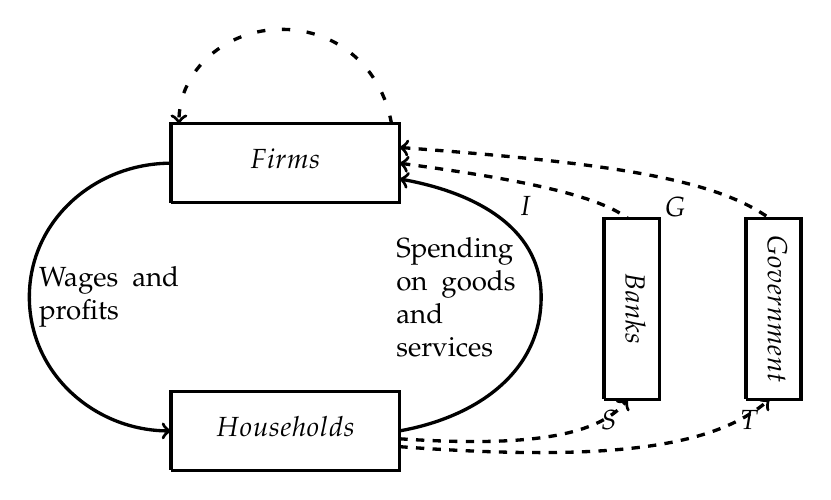
\begin{tikzpicture}[scale=1]

\node [above] at (3.25, 0.3) {$Households$};
\node [above] at (3.25, 3.7) {$Firms$};
\node [below] at (6.3, 3.6) {$I$};
\node [below] at (8.2, 3.6) {$G$};
\node at (7.7, 2.05){\rotatebox{-90}{$Banks$}};
\node at (9.5, 2.05){\rotatebox{-90}{$Government$}};
\node at (0, 2.2) [align = left, right] {Wages \ and \\ profits};
\node at (6.3, 2.2) [align = left, left] {Spending \\ on \ goods \\ and \\ services};

\draw [very thick] (1.8, 0) -- (4.7, 0) -- (4.7, 1) -- (1.8, 1) -- (1.8, 0);
\draw [very thick] (1.8, 3.4) -- (4.7, 3.4) -- (4.7, 4.4) -- (1.8, 4.4) -- (1.8, 3.4);
\draw [very thick, ->] [loosely dashed] (4.6, 4.4) to [out=100, in=0] (3.2, 5.6) to [out=180, in=90] (1.9, 4.4);
\draw [very thick] (7.3, 0.9) -- (8, 0.9) -- (8, 3.2) -- (7.3, 3.2) -- (7.3, 0.9);
\draw [very thick] (9.1, 0.9) -- (9.8, 0.9) -- (9.8, 3.2) -- (9.1, 3.2) -- (9.1, 0.9);

\draw [very thick, ->] (1.8, 3.9) to [out=-180, in=90] (0, 2.2) to [out=-90, in=180] (1.8, 0.5);
\draw [very thick, ->] (4.7, 0.5) to [out=10, in=-90] (6.5, 2.2) to [out=90, in=-10] (4.7, 3.7);
\draw [very thick, ->] [dashed] (4.7, 0.4) ..controls (6.2, 0.3) and (7.2, 0.4) ..(7.6, 0.9) node [below left] {$S$};
\draw [very thick, ->] [dashed] (4.7, 0.3) ..controls (7.4, 0.1) and (8.7, 0.3) ..(9.4, 0.9) node [below left] {$T$};
\draw [very thick, <-] [dashed] (4.7, 3.9) ..controls (6.2, 3.7) and (7.2, 3.5) ..(7.6, 3.2);
\draw [very thick, <-] [dashed] (4.7, 4.1) ..controls (7.4, 3.9) and (8.7, 3.7) ..(9.4, 3.2);

\end{tikzpicture}
\captionsetup{labelformat=empty} 
\textbf{\caption{Circular Flow Diagram}}
\end{figure}
\end{frame}


\begin{frame}
\frametitle{Other Measures of Income}

\begin{itemize}

\item \textit{Gross National Product (GNP)}: Total income earned by a nation's citizens. It includes income earned by citizens who live abroad and excludes earnings by foreigners working within country.
\item \textit{Net National Product (NNP)}: Total income minus depreciation. 
\item \textit{National Income}:  Total income earned in the production of goods and services. It excludes indirect business taxes and includes subsidies given to businesses.
\item \textit{Personal Disposable Income}: Total income received by households and non-corporate businesses minus personal taxes.
\pause
\item  GVA  at factor cost + (Production taxes less Production subsidies) = GVA at basic  prices
\item  GDP  at market prices = GVA at basic prices + Product taxes- Product subsidies

\end{itemize}
\end{frame}



\begin{frame}
\frametitle{Components of GDP}
To understand how the economy is using its scarce resources, economists study
the composition of GDP among various types of spending. To do this, GDP (which
we denote as $Y$) is divided into four components: consumption ($C$), investment ($I$),
government purchases ($G$), and net exports ($NX$): \\
$Y = C + I + G + NX$.
\end{frame}




\begin{frame}
\frametitle{Real Versus Nominal GDP}

If total spending is changing over time, one of the following must be true: \\
1. There is greater production of goods and services in the country.  \\
2. The price of the goods and services has risen. \\
To separate one from the other effect, we use \textit{real} GDP. \\
\pause

\vspace{3mm}

Nominal GDP uses current prices to place a value on the economy's production
of goods and services. Real GDP uses constant base-year prices to place a value on
the economy's production of goods and services
\end{frame}


\begin{frame}
\frametitle{Real and Nominal GDP}
 Example
\\
\begin{center}
\begin{tabular}{ ccccc } 
 \hline
 Year & Price (per kg) & Quantity & Price  & Quantity \\
 %\hline
& of Rice & of Rice & of Fish & of Fish \\
\hline
2015 & 10 & 1000 & 20 & 500 \\
2016 & 20 & 1500 & 30 & 1000\\
2017 & 30 & 2000 & 40 & 1500\\
 \hline
\end{tabular}
\end{center}

\end{frame}

\begin{frame}
\frametitle{GDP Deflator}
Nominal GDP reflects both the quantities of goods and services
the economy is producing and the prices of those goods and services. \\
By contrast, by holding prices constant at base-year levels, real GDP reflects only the
quantities produced. \\


From these two statistics, we can compute a third, called the
GDP deflator, which reflects only the prices of goods and services. \\

$ \text{GDP Deflator} = \frac{\text{Nominal GDP}}{\text{Real GDP}}*100$
\end{frame}


\begin{frame}

\frametitle{Exercise}

Below are some data from the land of milk and honey. \\
\linespread{1}
\begin{center}
\begin{tabular}{ ccccc } 
 \hline
 Year & Price (per kg) & Quantity & Price (per 100g)  & Quantity \\
 %\hline
& of Milk & of Milk & of Honey & of Honey \\
\hline
2015 & 70 & 100 & 140 & 50 \\
2016 & 70 & 200 & 140 & 100 \\
2017 & 140 & 200 & 280 & 100 \\
 \hline
\end{tabular}
\end{center}
1. Calculate nominal GDP, real GDP, and GDP deflator (base: 2015). \\
2. Compute percentage change in nominal GDP, real GDP, GDP deflator. \\
3. Did economic well-being rise more in 2016 than in 2017? Explain.

\end{frame}

\begin{frame}
\frametitle{Exercise}
A farmer grows wheat, which he sells to a miller
for \$100. The miller turns the wheat into flour,
which he sells to a baker for \$150. The baker
turns the wheat into bread, which he sells to
consumers for \$180. Consumers eat the bread. \\


\vspace{3mm}

a. What is GDP in this economy? Explain. \\
b. Value added is defined as the value of a
producer's output minus the value of the
intermediate goods that the producer buys
to make the output. Assuming there are no
intermediate goods beyond those described
above, calculate the value added of each of
the three producers. \\
c. What is total value added of the three
producers in this economy? How does it
compare to the economy's GDP? Does this
example suggest another way of calculating
GDP?
\end{frame}

\section{Measurement of Price Level}
\begin{frame}
\frametitle{Consumer Price Index}
The consumer price index (CPI) is a measure of the overall cost of the goods and
services bought by a typical consumer. Each month, the Labour Bureau of India computes and reports the
consumer price index.
\end{frame}

\begin{frame}
\frametitle{Consumer Price Index}
Cookbook: \\
%\\
\textit{Fix the basket.} Determine which prices are most important to the typical consumer.
If the typical consumer buys more rice than wheat, then
the price of rice is more important than the price of wheat and,
therefore, should be given greater weight in measuring the cost of living. \\
\textit{Find the prices.} Find the prices of each of the goods and services in the basket
at each point in time. \\
\textit{Compute the basket's cost.} Use the data on prices to calculate the cost of the
basket of goods and services at different times. \\
\textit{Choose a base year and compute the index.} \\

\begin{center}
$ CPI = \frac{\text{Cost of the basket in current year}}{\text{Cost of the basket in base year}}*100$ \\
\end{center}


\textit{Compute the inflation.} \\
\begin{center}
$ \text{Inflation} = \frac{CPI_1 - CPI_0}{CPI_0}*100$
\end{center}

\end{frame}
%\end{frame}

\begin{frame}
\frametitle{Exercise}
\linespread{1}
\begin{center}
\begin{tabular}{ cccc } 
 \hline
  & Injera & Pizza & Ice Cream \\
 %\hline
%& of Milk & of Milk & of Honey & of Honey \\
\hline
2015 price & 140 & 280 & 70 \\
2015 quantity & 100 & 100 & 200 \\
2016 price & 140 & 420 & 140  \\
2016 quantity & 100 & 100 & 200 \\
 \hline
\end{tabular}
\end{center}

\begin{itemize}
\item Using a method similar to the consumer price
index, compute the percentage change in the
overall price level. 

\item If you were to learn that an ice-cream scoop
increased in size from 2015 to 2016, should
that information affect your calculation of the
inflation rate? If so, how?

\item If you were to learn that the ice cream store introduced
new flavours in 2016, should that information
affect your calculation of the inflation rate? If
so, how?
\end{itemize}

\end{frame}



\begin{frame}
\frametitle{Few Other Things}
\begin{itemize}
\item Differences between GDP Deflator \& CPI. 
\pause
\item Real and nominal interest rates. \\
 Real interest rate = nominal interest rate - inflation rate
\end{itemize}
\end{frame}




\end{document}